\thispagestyle{firstpage}

% --- Title block ---
\begin{tcolorbox}[
    colback=headerblue,
    colframe=headerblue,
    coltext=white,
    boxrule=0pt,
    arc=3pt,
    left=15pt,right=15pt,top=12pt,bottom=12pt,
    ]
    \begin{minipage}[t]{0.7\textwidth}
        {\Huge\bfseries Receiver Design Project}\\[4pt]
        {\Large Superheterodyne Receiver}\\[8pt]
        {\large Grant Saggars}\\[8pt]
    \end{minipage}
    \hfill
\end{tcolorbox}

\vspace{8pt}

\section{TUNING SOLUTION}
% --- Quick specs table ---
\begin{table}[H]
    \centering
    \begin{tabular}{|C{3.5cm}|C{4.3cm}|C{2.4cm}|C{4.2cm}|}
        \hline
        \rowcolor{medgray}
        \textbf{PARAMETER} & \textbf{VALUE (MHz)} & \textbf{VALUE ($\boldsymbol{\alpha}$)} & \textbf{ATTENUATION} \\
        \hline
        RF Band & 1250 MHz - 1550 MHz & & \\
        \hline
        $f_{0}^{\text{IF}}$\textsuperscript{\hyperref[sec:IF-center]{(reasoning below)}} & 320 MHz & & \\
        \hline
        LO Band\textsuperscript{\hyperref[eq:LO]{(see calc.)}} & 1570 MHz - 1870 MHz & & \\
        \hline
        \hline
        Image Band\textsuperscript{\hyperref[eq:image-derivation]{(see calc.)}} & 1890 MHz - 2190 MHz & 1.883 - 3.351 & 40 dB Minimum \\
        \hline
        $\omega_{3a}^m$\textsuperscript{\hyperref[eq:3a]{(see calc.)}} & 106.667 MHz & 59.19 & >60 dB \\
        \hline
        $\omega_{3b}^m$\textsuperscript{\hyperref[eq:3b]{(see calc.)}} & 945.0 MHz - 1095.0 MHz & 1.248 - 2.684 & 30 dB Minimum \\
        \hline
        $\omega_{3c}^m$\textsuperscript{\hyperref[eq:3c]{(see calc.)}} & 625.0 MHz - 775.0 MHz & 4.75 - 7.25 & >60 dB \\
        \hline
        $\omega_{3d}^m$\textsuperscript{\hyperref[eq:3d]{(see calc.)}} & 3460 MHz - 4060 MHz & 8.667 - 10.94 & >60 dB \\
        \hline
        $\omega_{3e}^m$\textsuperscript{\hyperref[eq:3e]{(see calc.)}} & 2820 MHz - 3420 MHz & 6.11 - 8.512 & >60 dB \\
        \hline
         $\omega_{2a}^m$\textsuperscript{\hyperref[eq:2a]{(see calc.)}} & 160.0 MHz & 38.83  & >60 dB \\
        \hline
         $\omega_{1a}^m$\textsuperscript{\hyperref[eq:1a]{(see calc.)}} & 320 MHz & 18.12 & >60 dB \\
        \hline
    \end{tabular}
\end{table}

\begin{tcolorbox}[featureBox, title=1.1 Selection of IF Center]
    \label{sec:IF-center}

    We compared both high-side and low-side tuning solutions, and chose to go with high-side. Our method for doing this involved first plotting spurrious sources and images for all potential IF center frequencies as their center frequency, shown in figure \ref{fig:normalized_freq_response}. This enabled us to select an IF center which balances the worst-case signals, the image $LO + IF$, and the $\omega_{3b}$ murphy signal $\frac{LO+IF}{2}$.

    \begin{figure}[H]
        \centering
        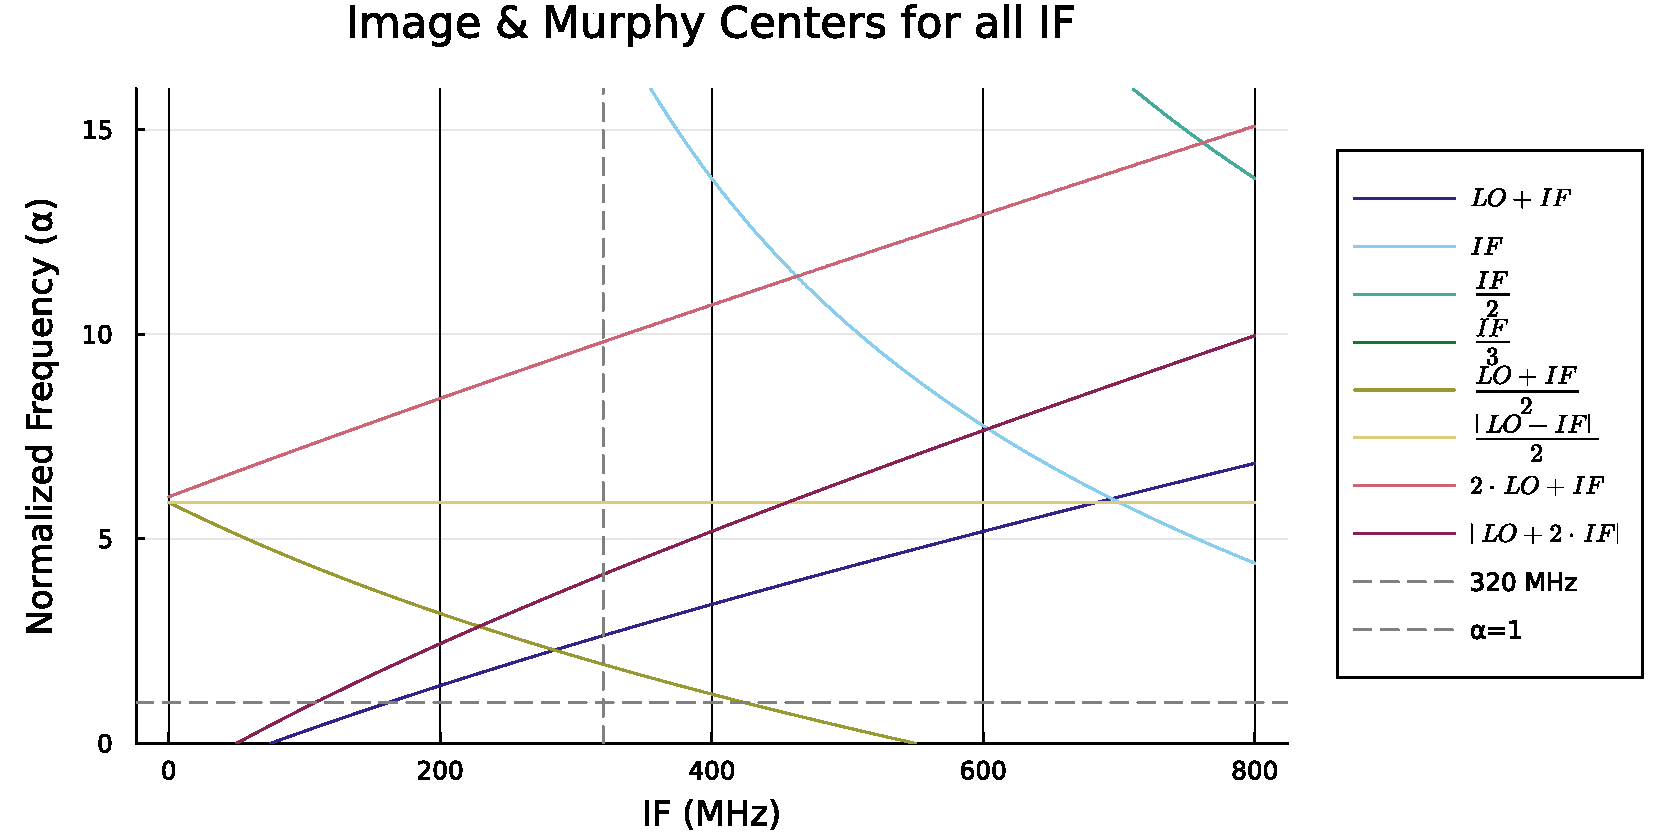
\includegraphics[width=0.6\textwidth]{../../assets/normalized_freq_response.pdf}
        \caption{For any given IF, the lowest alpha for each signal is desired. 1$\alpha$ maps to 30 dB of attenuation, the minimum allowable attenuation. We select 320 MHz, as it offers improved image attenuation at the cost of attenuation in murphy signals.}
        \label{fig:normalized_freq_response}
    \end{figure}

\end{tcolorbox}

\vspace{8pt}
\section{IF Filter Specification}

\begin{table}[H]
    \centering
    \begin{tabular}{|C{3.5cm}|C{4.3cm}|}
        \hline
        \rowcolor{medgray}
        \textbf{PARAMETER} & \textbf{VALUE} \\
        \hline
        Order & 3 \\
        \hline
        Type & Butterworth \\
        \hline
        Kind & Band \\
        \hline
        Center & 320 MHz \\
        \hline
        Bandwidth & 300 MHz \\
        \hline
        In/Out Impedance & Matched to 50 $\Omega$ \\
        \hline
        Insertion Loss & 1 dB \\
        \hline
        Max Input Power & 10 W \\
        \hline
    \end{tabular}
\end{table}

\begin{tcolorbox}[featureBox, title=2.1 Selection of IF Filter Order]

    \vspace{1em}
    Due to the narrow bandwidth, a butterworth filter is selected for its nearly linear phase-delay, and good dispersion. The FCC specification assigns our signals a 2.0 MHz bandwidth, which are no closer than 5.0 MHz. To determine a filter specification, we will express the spacing between stations in terms of its $\alpha$, to select a minimum roll-off.

    \vspace{1em}
    Let the upper and lower frequency bounds be denoted in terms of $f_c$,
    $$f_H(f_c) = f_c + 1\,\text{MHz} \qquad \text{and} \qquad f_L(f_c) = f_c - 1\,\text{MHz}$$

    \vspace{1em}
    And the center frequency as 
    $$f_0(f_c) = \sqrt{f_H(f_c) \cdot f_L(f_c)}$$

    \vspace{1em}
    Then we define:
    \begin{align*}
        \Delta(f_c) &= \frac{f_0(f_c)}{f_H(f_c) - f_L(f_c)}
                    &\alpha(f_c) = \left|\Delta(f_c) \cdot \left(\frac{f_c + \text{spacing}}{f_0(f_c)} - \frac{f_0(f_c)}{f_c + \text{spacing}}\right)\right| - 1 \tag{2.1}
    \end{align*}

    We find that, at worst, we filter signals at $3.96\alpha$ or further by 40 dB, which demands a 3rd order butterworth filter.

\begin{figure}[H]
  \centering
  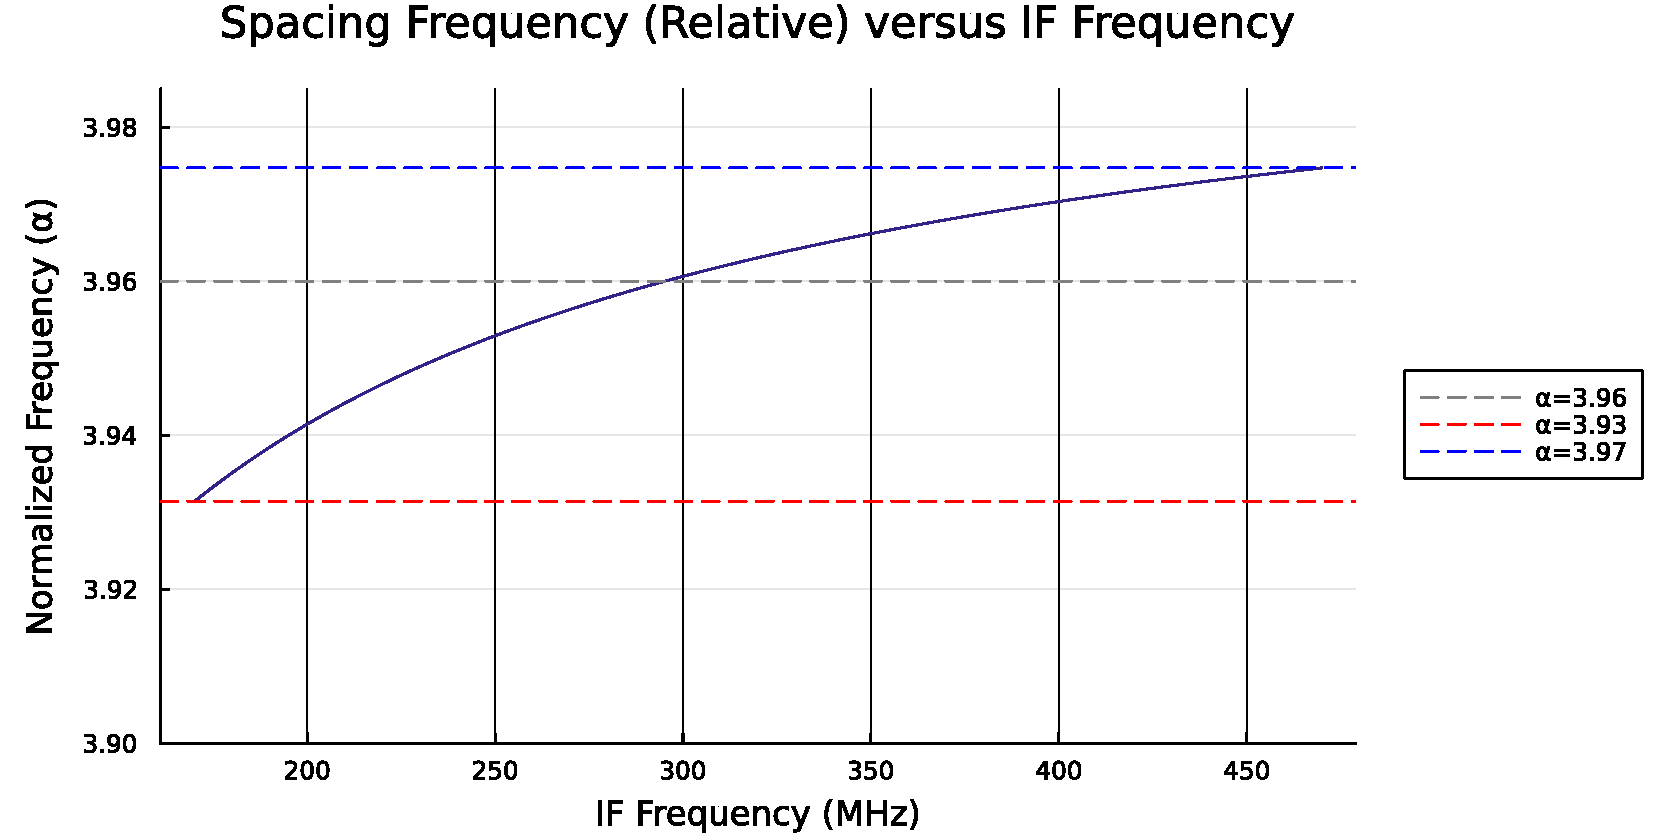
\includegraphics[width=0.6\textwidth]{../../assets/if_filter_gap.pdf}
  \caption{Filter response at $\alpha = f_c + 5$ MHz.}
  \label{fig:if_filter_gap}
\end{figure}

\end{tcolorbox}

\section{Local Oscillator Specification}

\begin{table}[H]
    \centering
    \begin{tabular}{|L{7cm}|L{8cm}|}
        \hline
        \rowcolor{medgray}
        \textbf{Parameter} & \textbf{Value} \\
        \hline
        Carrier Frequency & 1 GHz - 2 GHz \\
        \hline
        Carrier Power & 13 dBm min. \\
        \hline
        Accuracy & At least $\pm$64 ppm between $-25^\circ$ C to $85^\circ$ C \\
        \hline
        Harmonics and Spurs & -60 dBc maximum \\
        \hline
        Phase Noise & At most -110 dBc in a 1 Hz bandwidth at 1 kHz from the carrier frequency $f_{0}$ \\
        \hline
        Noise Floor & -155 dBm in a 1 Hz bandwidth \\
        \hline
        DC Power & +7 volts to +24 volts at 2 W typical to 2.5 W maximum \\
        \hline
        Efficiency\textsuperscript{\hyperref[eq:lo-efficiency]{(see calc.)}} & 0.01 typical (0.08 at max power) \\
        \hline
        Frequency Pulling (1.5:1 VSWR) & 1 MHz peak-to-peak \\
        \hline
        Frequency Pushing & 10 kHz/V max. \\
        \hline
    \end{tabular}
\end{table}

\begin{tcolorbox}[featureBox, title=3.1 Selection of LO Accuracy]
     IF port accuracy is specified in ppm, as a function of the LO oscillator frequency and given in eq. 3.1, and can range from 1570 MHz - 1870 MHz, specified in section 1. LO frequency error may be no more than 10\% of the IF bandwidth, as a rule of thumb.
     % \begin{equation}
     % \mathrm{ppm}(\Delta f_{0})\equiv 10^{6}\left( \frac{\Delta f_{r}(\mathrm{Hz})}{f_{0}(\mathrm{Hz})} \right) \tag{3.1}
     % \end{equation}
     
     \vspace{1em}
     The worst case scenario occurs at $f_{\text{LO}}=1570$ MHz, with a value of 64 ppm ppm\textsuperscript{\hyperref[eq:lo-accuracy]{(see calc.)}}. Thus, our specification must have accuracy better than ±64 ppm to ensure the $\pm1$ MHz frequency tolerance is met across the entire LO frequency range. Complete accuracy characteristics are shown in figure \ref{fig:accuracy}.

     \vspace{1em}
\begin{figure}[H]
  \centering
  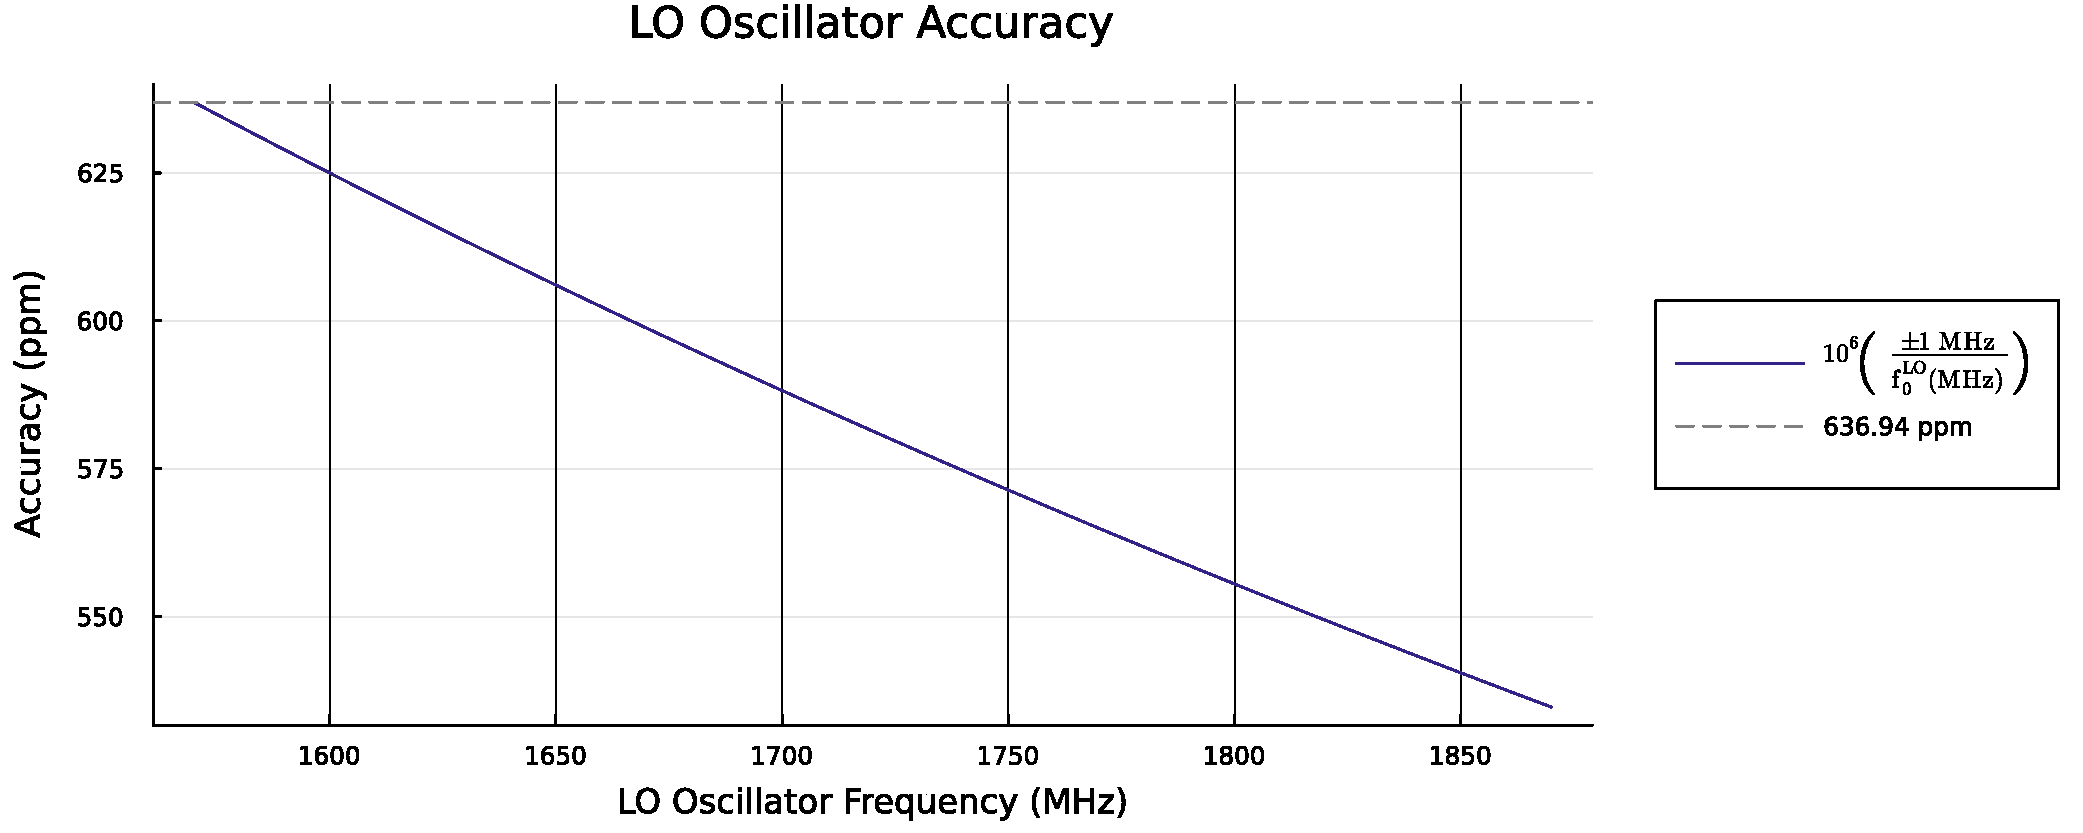
\includegraphics[width=0.8\textwidth]{../../assets/accuracy.pdf}
  \caption{Complete LO oscillator accuracy characteristics. The worst case is given at the highest LO frequency, labelled by a dashed line.}
  \label{fig:accuracy}
\end{figure}
\end{tcolorbox}


\newpage
\section{Appendix: Calculations}

\subsection{LO Bandwidth}
\label{eq:LO}
\begin{align*}
    f_{LO,L} &= f_{RF,L} + f_{IF} = 1250 + 320 = 1570 \mathrm{~MHz} \\
    f_{LO,H} &= f_{RF,H} + f_{IF} = 1550 + 320 = 1870 \mathrm{~MHz}
\end{align*}

\subsection{Normalized Frequency Parameter}

The normalized frequency parameter $\alpha$ is defined as:
\begin{align}
    \%\Delta &= \frac{f_{0}}{f_{H}-f_{L}} \\
    \alpha(f)&=\left| \%\Delta \left( \frac{f}{f_{0}}-\frac{f_{0}}{f} \right) \right| - 1
\end{align}

\subsection{Image Band}
\label{eq:image-derivation}

\begin{align}
f_{image,L} &= f_{LO,L} + f_{IF} = 1890\,\text{MHz} \\
f_{image,H} &= f_{LO,H} + f_{IF} = 2190\,\text{MHz}
\end{align}

Range: $\alpha \in [1.883, 3.351]$

\subsection{Murphy Spectrum - $\omega_{1a}^m$}
\label{eq:1a}

\begin{equation}
\omega_{1a}^m = f_{IF} = 320\,\text{MHz}
\end{equation}

Range: $\alpha = 18.12$

\subsection{Murphy Spectrum - $\omega_{2a}^m$}
\label{eq:2a}

\begin{equation}
\omega_{2a}^m = \frac{f_{IF}}{2} = 160\,\text{MHz}
\end{equation}

Range: $\alpha = 38.83$

\subsection{Third-Order Murphy Frequencies}

\subsubsection{Murphy Spectrum - $\omega_{3a}^m$}
\label{eq:3a}

\begin{equation}
\omega_{3a}^m = \frac{f_{IF}}{3} = 106.667\,\text{MHz}
\end{equation}

Range: $\alpha = 59.19$

\subsubsection{Murphy Spectrum - $\omega_{3b}^m$}
\label{eq:3b}

\begin{align}
\omega_{3b,L}^m &= \frac{f_{LO,L} + f_{IF}}{2} = 945\,\text{MHz} \\
\omega_{3b,H}^m &= \frac{f_{LO,H} + f_{IF}}{2} = 1095\,\text{MHz}
\end{align}

Range: $\alpha \in [1.248, 2.684]$

\subsubsection{Murphy Spectrum - $\omega_{3c}^m$}
\label{eq:3c}

\begin{align}
\omega_{3c,L}^m &= \frac{|f_{LO,L} - f_{IF}|}{2} = 625\,\text{MHz} \\
\omega_{3c,H}^m &= \frac{|f_{LO,H} - f_{IF}|}{2} = 775\,\text{MHz}
\end{align}

Range: $\alpha \in [4.75, 7.25]$

\subsubsection{Murphy Spectrum - $\omega_{3d}^m$}
\label{eq:3d}

\begin{align}
\omega_{3d,L}^m &= 2f_{LO,L} + f_{IF} = 3460\,\text{MHz} \\
\omega_{3d,H}^m &= 2f_{LO,H} + f_{IF} = 4060\,\text{MHz}
\end{align}

Range: $\alpha \in [8.667, 10.94]$

\subsubsection{Murphy Spectrum - $\omega_{3e}^m$}
\label{eq:3e}

\begin{align}
\omega_{3e,L}^m &= |2f_{LO,L} - f_{IF}| = 2820\,\text{MHz} \\
\omega_{3e,H}^m &= |2f_{LO,H} - f_{IF}| = 3420\,\text{MHz}
\end{align}

Range: $\alpha \in [6.11, 8.512]$

\subsubsection{LO Oscillator Accuracy (Worst Case)}
\label{eq:lo-accuracy}

\begin{equation}
    \mathrm{ppm}(\Delta f_{0})\equiv 
    10^{6}\left( \frac{0.1 \cdot \Delta f_{r}(\mathrm{Hz})}{f_{0}(\mathrm{Hz})} \right) 
    =10^{6}\left( \frac{\pm \mathrm{1~MHz}}{\mathrm{1570~MHz}} \right) \approx 64\mathrm{~ppm}
\end{equation}

\subsubsection{LO Oscillator Efficiency}
\label{eq:lo-efficiency}

\begin{equation}
    \mathrm{\frac{10^{(13/10)}~mW}{2~W}} = \mathrm{\frac{20~mW}{2000~mW}} = 0.01
\end{equation}

\section{Appendix: Other}

\begin{tcolorbox}[featureBox, title=a.1]

    We also consider the low-side tuning solution for the receiver, which nets similar, but slightly worse results. As expected, the image and $2f_{LO} + f_{IF}$ are the most concerning RF signals. The best we could achieve for the image while attenuating this murphy signal by 30dB is approximately $1.65\alpha$ from the RF signal, which is $\sim13\%$ closer.

    \begin{figure}[H]
        \centering
        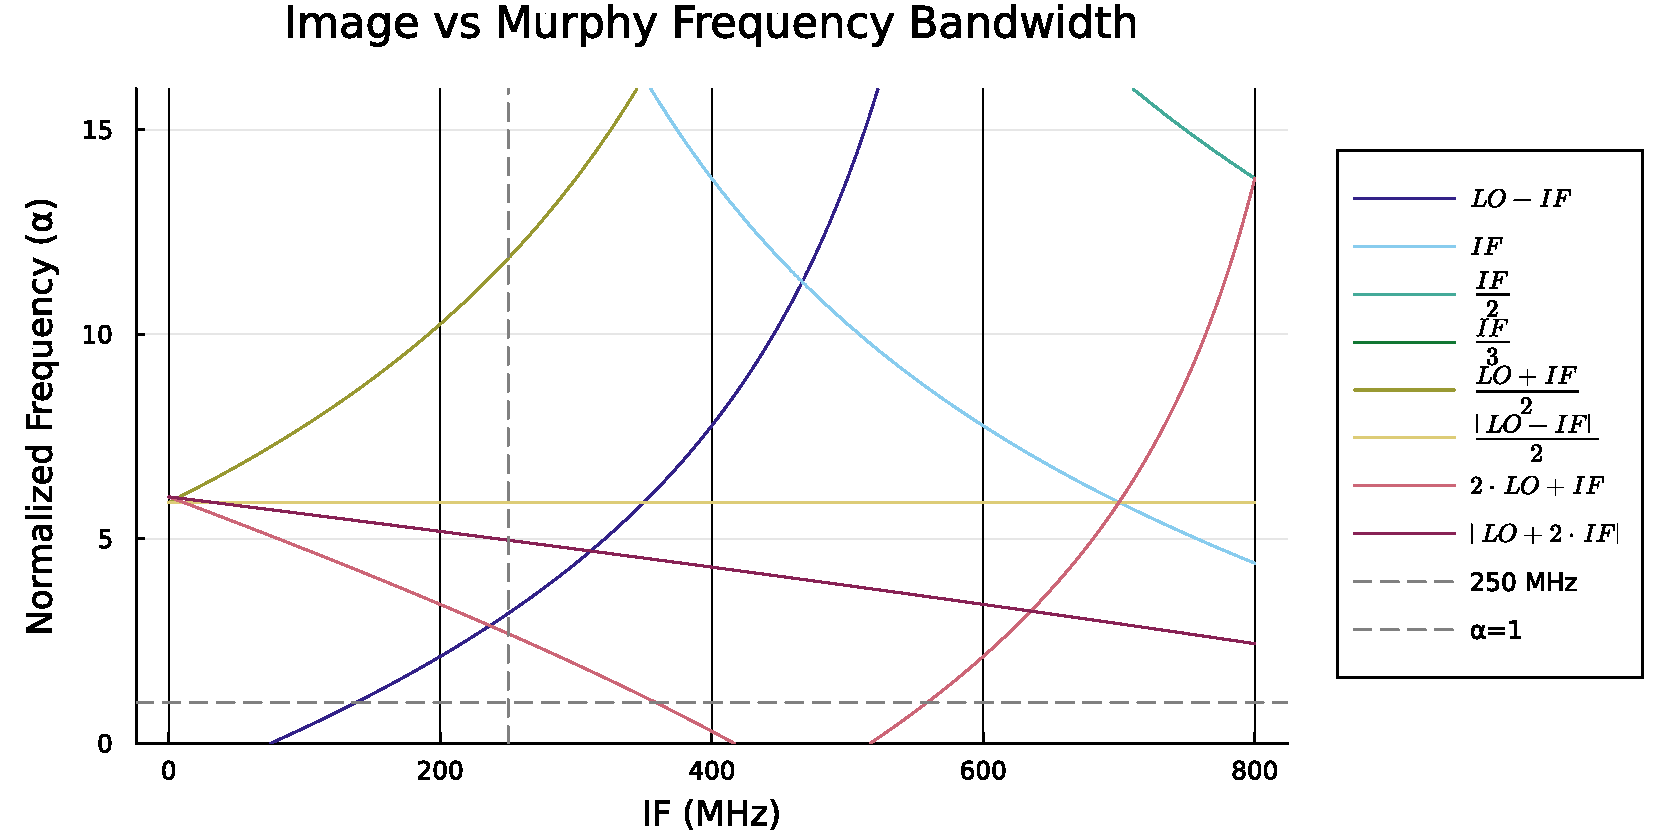
\includegraphics[width=0.6\textwidth]{../../assets/normalized_freq_response_lowside.pdf}
    \end{figure}

\end{tcolorbox}
